\chapter{Cronograma das atividades}\label{cha:cronograma}

Este apêndice apresenta o cronograma das atividades durante todo o desenvolvimento dessa pesquisa e das etapas que ainda
estão por vir. Cada atividade está numerada no cronograma e explicada em detalhe abaixo.

\begin{figure}[htb]
  \begin{center}
      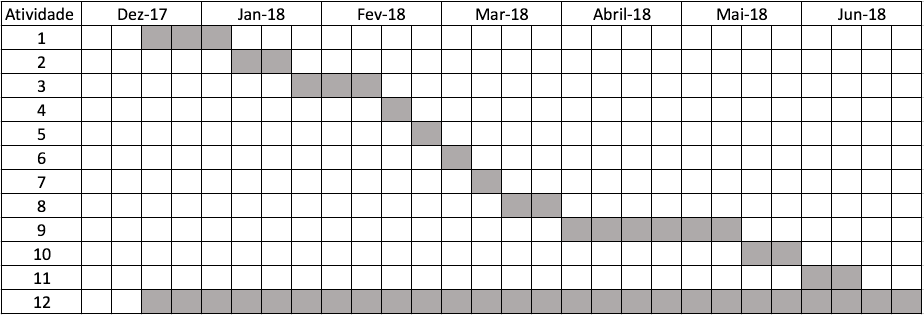
\includegraphics[scale=0.5]{./Figuras/cronograma.png}
  \end{center}
  \legend{Fonte: \citeonline{gasparini2003interface}}
\end{figure}

\begin{enumerate}
\item Estudo dos Sistemas de Recomendação aplicados em Ambientes Virtuais de Aprendizagem
\item Estudo dos Sistemas de Recomendação Sensíveis ao Tempo
\item Análise de como aplicar os Sistemas de Recomendação Sensíveis ao Tempo em Ambientes Virtuais de Aprendizagem
\item Estudo das formas de avaliação de Sistema de Recomendação
\item Estudo das métricas para avaliação de Sistemas de Recomendação
\item Estudo das formas de avaliação de Sistema de Recomendação em Ambientes Virtuais de Aprendizagem
\item Identificar as características do AdaptWeb\textsuperscript{\textregistered}
\item Estudo para decidir o algoritmo a ser utilizado
\item Identificar os pontos de alteração no AdaptWeb\textsuperscript{\textregistered}
\item Definir a forma de avaliação a ser realizada e as métricas utilizadas
\item Implementar a proposta no AdaptWeb\textsuperscript{\textregistered}
\item Realizar o experimento para avaliação da proposta
\item Analisar os resultados do experimento
\item Escrever a dissertação
\end{enumerate}
